\documentclass[times, utf8, zavrsni]{fer}
\usepackage{booktabs}
\usepackage{amsmath}
\usepackage{graphicx}

\usepackage{listings}
\usepackage{color}
\usepackage{setspace}
%\definecolor{dkgreen}{rgb}{0,0.6,0}
\definecolor{gray}{rgb}{0.5,0.5,0.5}
%\definecolor{mauve}{rgb}{0.58,0,0.82}
\definecolor{black}{rgb}{0.0, 0.0, 0.0}

\renewcommand\lstlistingname{Ispis}
\renewcommand\lstlistlistingname{Popis ispisa}

\lstset{
mathescape,
frame=tb,
language=C,
aboveskip=3mm,
belowskip=3mm,
showstringspaces=false,
columns=flexible,
basicstyle={\small\ttfamily},
numbers=left,
numberstyle=\small\color{black},
keywordstyle=\color{black},
commentstyle=\color{black},
stringstyle=\color{black},
breaklines=true,
breakatwhitespace=true,
tabsize=2
}

\begin{document}

% TODO: Navedite broj rada.
\thesisnumber{3253}

% TODO: Navedite naslov rada.
\title{GPU implementacija vremenski i memorijski učinkovitoga paralelnog algoritma za poravnanje slijedova}

% TODO: Navedite vaše ime i prezime.
\author{Marija Mikulić}

\maketitle

% Ispis stranice s napomenom o umetanju izvornika rada. Uklonite naredbu \izvornik ako želite izbaciti tu stranicu.
\izvornik

% Dodavanje zahvale ili prazne stranice. Ako ne želite dodati zahvalu, naredbu ostavite radi prazne stranice.
\zahvala{Hvala Miletu što me motivirao da se posvetim računarstvu, na ukazanom povjerenju, na prenesenom znanju i ponajviše na strpljenju.}

\tableofcontents

\listoftables

\listoffigures

% dodati u table of contents
\lstlistoflistings

\chapter{Uvod}

\indent

Od svojih začetaka u 1940-ima, računala su postupno postala dio naše svakodnevice. To je područje ljudskog djelovanja koje se najbrže mijenja i evoluira. Ta evolucija se događa velikim dijelom zbog toga što se računala sve više i na sve više različitih načina primjenjuju u raznim područjima ljudskog djelovanja.

Jedno od tih područja je i biologija. U biologiji su za neke probleme, poput poravnavanja proteina i DNK, računala ključni alat za dolaženje do novih spoznaja. Iz te neodvojive veze nastalo je cijelo područje istraživanja koje nazivamo bioinformatika.

Biolozi ulažu velike napore u proučavanje našeg građevnog materijala, proteina i gena koji nas tvore. Proučavanje ovih molekula pokazalo se kao vrlo bitno i potencijalno vrlo korisno.

Primjerice, ako bismo mogli manipulirati svojom DNK, mogli bismo ukloniti iz svojih gena mnoge bolesti i sindrome koji danas, nažalost, pogađaju mnoge ljude.

Naravno, to otvara vrata i mnogim drugim stvarima te je predmet brojnih etičkih i filozofskih rasprava, ali prvotni cilj znanosti jest nastojati otkriti kako funkcionira svijet oko nas. Stoga nam je vrlo zanimljivo proučavati kako, u svojoj srži, funkcioniramo mi sami.

Iz te znatiželje i iz činjenice da su u biološkim molekulama spremljeni gigabajti informacija, pojavila se potreba za razvijanjem algoritama kojima bi se moglo učinkovito obrađivati tolike količine informacija. Kao jedan od ključnih problema nametnuo se problem poravnavanja molekula proteina i DNK.

Konkretan problem kojim se bavi ovaj završni rad jest poravnavanje jednog proteina s listom proteina. Odnosno, zanima nas koliko je neki protein udaljen od svakog od \textit{n} proizvoljnih proteina. Ovaj rad opisuje rješenje toga problema algoritmom koji koristi predmetačni račun i Needleman-Wunschov algoritam.

Poglavlje 2 opisuje općenito problem poravnavanja struktura. U poglavlju 3 izložen je Needleman-Wunschov algoritam, a u poglavlju 4 predmetačni račun.
Poglavlje 5 opisuje tehnologiju CUDA, a poglavlje 6 specifičnosti implementacije, dok se u poglavlju 7 izlažu dobiveni rezultati. Poglavlje 8 posvećeno je zaključku rada.


\chapter{Poravnavanje struktura}
\indent

Problem kojim se bavi ovaj rad jest problem poravnavanja proteina za potrebe biologije. Svrha tog poravnavanja jest ustanoviti područja sličnosti između proteina, jer ona mogu indicirati funkcijsku, strukturalnu ili evolucijsku vezu između proteina.

Za potrebe informatike, ovaj problem se može svesti na problem poravnavanja nizova znakova. Za ilustraciju, zamislimo da se nizovi koje poravnavamo stave jedan ispod drugog. U tom slučaju, cilj je tako postaviti znakove nizova da oni izgledaju najsličnije moguće.

Razlikujemo dvije vrste poravnavanja: globalno i lokalno.

Globalno poravnavanje je postupak kojim se jedan niz preslikava na drugi od početka do kraja. Pri tome je dozvoljeno u bilo koji niz umetnuti prazninu na proizvoljno mjesto, osim na prvo i posljednje. Ukoliko je jedan niz znatno dulji od drugog, ovakvo poravnanje može za posljedicu imati umetanje velikog broja praznina u kraći niz.

Za razliku od globalnog, lokalno poravnanje ne vodi računa o tome da se iskoriste svi znakovi oba niza. Ovdje je cilj poravnati jedan niz na dio drugoga na način da taj niz i dio drugog na koji je poravnan budu najsličniji.

\section{Ocjenjivanje procjepa}

\indent
%TODO zavrsiti
Praznine koje se pojavljuju u nizovima znakova zapravo predstavljaju procjepe



\begin{figure}[ht!]
\centering
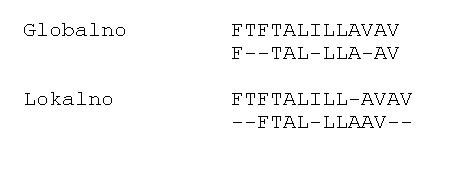
\includegraphics[width=90mm]{poravnanje.png}
\caption{Primjer globalnog i lokalnog poravnanja dvaju nizova}
\label{poravnanje}
\end{figure}

\chapter{Needleman-Wunschov algoritam}
\indent

Poznat još i kao algoritam optimalnog poravnanja, Needleman-Wunschov algoritam koristi se za globalno poravnavanje slijedova. To je prvi algoritam koji je primijenio dinamičko programiranje na problem poravnanja slijedova u biologiji.

Za ilustraciju rada algoritma poslužit će primjer poravnanja DNK slijedova \textit{AGACTAGTTAC} i \textit{CGAGACGT}.
Nad abecedom (u ovom slučaju \{A, C, G, T\}) definira se \textit{matrica sličnosti} za svaki par elemenata abecede, \textbf{S(a, b)}, kojom se boduje poravnanje ta dva elementa. Dodatno, funkcijom \textit{d} kažnjava se umetanje praznine u gornji ili donji slijed.

Neka je zadana sljedeća matrica sličnosti \textbf{S}:
\begin{center}
\begin{tabular}{r | r r r r}
 & \textbf{A} & \textbf{G} & \textbf{C} & \textbf{T} \\
\hline
\textbf{A} & 10 & -1 & -3 & -4\\
\textbf{G} & -1 & 7 & -5 & -3\\
\textbf{C} & -3 & -5 & 9 & 0\\
\textbf{T} & -4 & -3 & 0 & 8\\
\end{tabular}
\end{center}
Usto, neka je vrijednost funkcije kazne \textit{d} = 5. Tada bi poravnanje:
\begin{center}
\begin{tabular}{c c c c c c c c c c c }
A & G & A & C & T & A & G & T & T & A & C \\
C & G & A & - & - & - & G & A & C & G & T \\
\end{tabular}
\end{center}
imalo broj bodova 1: S(A, C) + S(G, G) + S(A, A) + 3 $\cdot$ d + S(G, G) + S(T, A) + S(T, C) + S(A, G) + S(C, T) = -3 + 7 + 10 - (3 $\cdot$ 5) + 7 + -4 + 0 + -1 + 0 = 1

\section{Algoritam}

\indent

Cilj Needleman-Wunschovog algoritma jest pronaći optimalno poravnanje neka dva slijeda A i B, odnosno ono poravnanje koje u obzir uzima sve znakove oba niza i usto ima najviši broj bodova s obzirom na sva moguća poravnanja (dozvoljeno je postojanje više rješenja s istim brojem bodova).

Označimo s \textit{n} duljinu slijeda A i s \textit{m} duljinu slijeda B. Za potrebe pronalaska optimalnog globalnog rješenja potrebno je alocirati dvodimenzionalnu matricu dimenzija \textit{n} $\times$ \textit{m}. Svaki redak matrice predstavlja znak u slijedu A, a svaki stupac predstavlja znak u slijedu B. Element matrice \textit{F$_{\textbf{ij}}$}, gdje je \textit{i} indeks retka, a \textit{j} indeks stupca, predstavlja broj bodova za poravnanje prvih \textit{i} znakova slijeda A i prvih \textit{j} znakova slijeda B.

Pošto tražimo optimalno globalno poravnanje, želimo biti sigurni da će poravnanje krenuti od prvog znaka slijeda A i prvog znaka slijeda B. Zbog toga se postavljaju sljedeći početni uvjeti:
\begin{center}
\textit{F$_{0j}$} = \textit{d $\times$ j}, \textit{i} = 0 ... \textit{n-1}\\
\textit{F$_{i0}$} = \textit{d $\times$ i}, \textit{i} = 0 ... \textit{m-1}
\end{center}
Svi ostali elementi matrice računaju se prema formuli:
\begin{center}
$$
F_{i,j} = \textit{max}\left\{
	\begin{array}{lr}
		F_{i-1,j-1} + S(A_{i}, B_{j}) \\
		F_{i, j-1} + d \\
		F_{i-1, j} + d
	\end{array}
\right.
$$
\end{center}

Nakon što su izračunati svi elementi matrice, element \textit{F$_{nm}$} sadrži broj bodova optimalnog globalnog poravnanja.

Pseudokod algoritma dan je u ispisu:

\begin{singlespace}
\begin{lstlisting}[caption={Needleman-Wunschov algoritam},label={needleman_wunsch}]
za svaki i od 0 do duljina(A):
	F[i, 0] = d * i
za svaki j od 0 do duljina(B):
	F[0, j] = d * j
za svaki i od 1 do duljina(A):
	za svaki j od 1 do duljina(B):
		bez_praznine = F[i - 1, j - 1] + S[A[i], B[i]]
		praznina_dolje = F[i - 1, j] + d
		praznina_gore = F[i, j - 1] + d
		F[i, j] = max(bez_praznine, praznina_dolje, praznina_gore)
\end{lstlisting}
\end{singlespace}

\section{Afina funkcija kazne}
\indent

Opisani algoritam kao funkciju kazne koristi konstantnu vrijednost. Međutim, u primjeni ovog algoritma na poravnanje bioloških struktura, proteina i nizova DNK, potrebno ga je modificirati. Naime, praznine koje se umeću predstavljaju mutacije, a veća je vjerojatnost da se dogodila jedna mutacija nad nekim podslijedom nego nekoliko mutacija duljine 1 zaredom. Stoga se definira afina funkcija kazne, koja za produljenje podslijeda praznina dodjeljuje manju kaznu nego za otvaranje novog podslijeda.

\subsection{Formalna definicija Needleman-Wunschovog algoritma s afinom funkcijom kazne}

\indent

Za verziju algoritma s afinom funkcijom kazne potrebno

\chapter{Predmetačni račun}

Problem predmetačnog računa definira se pomoću niza A = \{a$_{0}$, a$_{1}$, a$_{2}$, ..., a$_{n-1}$\} i općenitog binarnog operatora $\oplus$. Cilj je generirati niz B = \{0, 0 $\oplus$ a$_{0}$, 0 $\oplus$ a$_{0}$ $\oplus$ a$_{1}$, ..., 0 $\oplus$ a$_{0}$ $\oplus$ ... $\oplus$ a$_{n-2}$\}.

Ovaj se problem pojavljuje često kao usko grlo u raznovrsnim problemima. Neki od njih su:
\begin{itemize}
\item leksička usporedba nizova znakova (npr. određivanje da niz "strategija" dolazi ispred niza "strateški" u rječniku)
\item paralelno ostvarenje \textit{radix-sort} i \textit{quick-sort} algoritama
\item određivanje vidljivosti točaka u 3D krajoliku – uz operator \textit{max}
\item zbrajanje s brojevima višestruke (proizvoljne) preciznosti
\item alokacija procesora/memorije
\item pretraživanje regularnih izraza (npr. u implementaciji \textit{grep} naredbe u \textit{UNIX}-u)
\item izvedba nekih operacija nad stablima (npr. dubina svakog čvora u stablu)
\end{itemize}

\section{Primjer}

Za ilustraciju problema, pogledajmo slijedeći primjer:

Zadan je niz A:
\begin{center}
\begin{tabular}{| r | r | r | r | r | r | r | r | r |}
\hline
indeks & 0 & 1 & 2 & 3 & 4 & 5 & 6 & 7 \\
\hline
vrijednost & 5 & 3 & -8 & 4 & 12 & 6 & -9 & 1\\
\hline
\end{tabular}
\end{center}

Ako je binarni operator "+", tada je cilj dobiti niz B:
\begin{center}
\begin{tabular}{| r | r | r | r | r | r | r | r | r |}
\hline
indeks & 0 & 1 & 2 & 3 & 4 & 5 & 6 & 7 \\
\hline
vrijednost & 0 & 5 & 8 & 0 & 4 & 16 & 22 & 13\\
\hline
\end{tabular}
\end{center}

Gore navedeni primjer opisuje isključivi predmetačni račun. To znači da za element b$_{i}$ (\textit{i} = 0..\textit{n}) niza \textit{B} u obzir uzimamo elemente niza \textit{A} čiji je indeks manji od \textit{i}, a b$_{0}$ popunimo neutralnim elementom (primjerice, za zbrajanje je to 0).

Druga vrsta predmetačnog računa jest uključivi predmetačni račun, koji za izračun elementa b$_{i}$ koristi sve elemente od a$_{0}$ do a$_{i}$, uključivo. Za gore navedeni primjer, niz B bi izgledao ovako:
\begin{center}
\begin{tabular}{| r | r | r | r | r | r | r | r | r |}
\hline
indeks & 0 & 1 & 2 & 3 & 4 & 5 & 6 & 7\\
\hline
vrijednost & 5 & 8 & 0 & 4 & 16 & 22 & 13 & 14\\
\hline
\end{tabular}
\end{center}

Isključivi predmetačni račun se jednostavno generira iz uključivog tako da se svi elementi pomaknu za jedno mjesto udesno, a kao nulti element se doda neutralni element.


\section{Algoritam}

\indent

Predmetačni račun je jedan od algoritama koji se čine inherentno sekvencijalnima, ali za koje postoji učinkovita paralelna implementacija.

\subsection{Sekvencijalni algoritam}

\indent

Sekvencijalna implementacija ovog algoritma je trivijalna i svodi se na dinamičko programiranje. Verzija algoritma sa binarnim operatorom "+" dana je u ispisu:

%pseudokod
\begin{singlespace}
\begin{lstlisting}[caption={Predmetačni zbroj},label={predmetacni zbroj}]
b[0] := 0
za svaki k od 1 do n-1
	b[k] := a[k-1] + b[k-1]
\end{lstlisting}
\end{singlespace}

\subsection{Paralelni algoritam}

\indent
%dodati literaturu

Učinkovita paralelna implementacija predmetačnog računa temelji se na radu Blellocha i koristi balansirano stablo. Ideja je izgraditi balansirano binarno stablo nad ulaznim podacima te njegovim obilaskom do listova do korijena pa od korijena do listova napraviti račun.

Binarno stablo s \textit{n} listova ima dubinu \textit{d = log$_{2}$n}, a svaka dubina ima \textit{2$^{d}$} čvorova. Ako izvodimo jedan izračun po čvoru, u jednom obilasku stabla izvodimo \textit{O(n)} izračuna. Ovo binarno stablo nije fizički implementirano, nego je koncept koji koristimo kako bismo odredili što je zadatak svake dretve u obilasku stabla, a svi izračuni izvode se nad ulaznim nizom podataka.

Izračun se izvodi u dvije faze: reduciranje i predtraženje.

U fazi reduciranja, stablo se obilazi od listova do korijena i izvode se djelomični izračuni, te na kraju ove faze korijen stabla sadrži izračun za sve čvorove u stablu.

Slika i ispis predstavljaju fazu reduciranja na gore navedenom primjeru.

\begin{figure}[ht!]
\centering
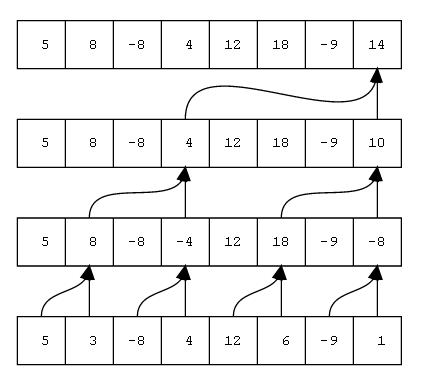
\includegraphics[width=90mm]{redukcija.png}
\caption{Faza redukcije}
\label{redukcija}
\end{figure}

\begin{singlespace}
\begin{lstlisting}[caption={Faza reduciranja}, label={reduciranje}]
za svaki d od 0 do log$_{2}$n - 1:
	za svaki k od 0 do n - 1 s korakom 2$^{d+1}$ u paraleli:
		a[k + 2$^{d+1}$ - 1] = a[k + 2$^{d}$ - 1] + a[k + 2$^{d+1}$ - 1]
\end{lstlisting}
\end{singlespace}

U fazi predtraženja stablo se obilazi od korijena do listova i koriste se djelomični izračuni iz faze reduciranja kako bismo izveli predmetačni račun za svaki element.

U korijen stabla se umetne neutralni element. Zatim, u svakom koraku čvor trenutne razine svom lijevom djetetu preda svoju vrijednost, a zbroj svoje vrijednosti i prethodne vrijednosti lijevog djeteta preda desnom djetetu.

Slika i ispis predstavljaju fazu predtraženja na gore navedenom primjeru.
\pagebreak

\begin{figure}[Htb]
\centering
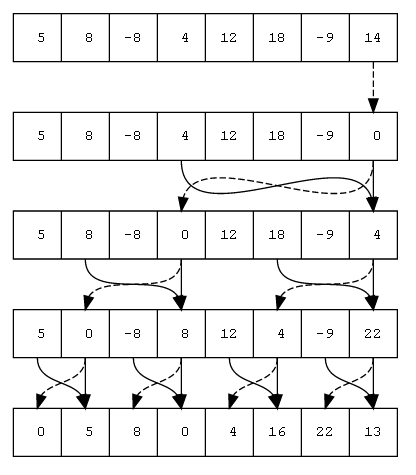
\includegraphics[width=90mm]{predtrazenje.png}
\caption{Faza predtraženja}
\label{predtrazenje}
\end{figure}

\begin{singlespace}
\begin{lstlisting}[caption={Faza predtraženja}, label={prescan}]
a[n-1] = 0
za svaki d od log$_{2}$n - 1 do 0:
	za svaki k od 0 do n - 1 s korakom 2$^{d}$ + 1:
		temp = a[k + 2$^{d}$ - 1]
		a[k + 2$^{d}$ - 1] = a[k + 2$^{d+1}$ - 1]
		a[k + 2$^{d+1}$ - 1] = temp + a[k + 2$^{d+1}$ - 1]
\end{lstlisting}
\end{singlespace}

\chapter{CUDA tehnologija}
\indent

Grafičke kartice su prvotno dizajnirane kao grafički ubrzivači i podržavale su cjevovode točno određenih funkcija. No, u 1990-im godinama doživjele su dramatičan razvoj i postajale sve više programabilne. NVIDIA, tvrtka koja je i skovala termin GPU (\textit{graphics processing unit} - \textit{grafička procesna jedinica}), svoj je prvi GPU proizvela 1999. Od tad su moć te tehnologije, osim proizvođača računalnih igara i umjetnika, prepoznali i mnogi istraživači te ju počeli koristiti za svoje potrebe.

Međutim, u to doba je bilo potrebno "prevariti" grafičku karticu koju se htjelo iskoristiti, to jest, trebalo podatke pretočiti u probleme koji se mogu prikazati trokutima i poligonima. Kako bi se to izbjeglo, razvio se GPGPU (\textit{general purpose graphics processing unit} - \textit{grafička procesna jedinica opće namjene}).

Uskoro su se pojavile i prilagodbe općih programskih jezika za novonastalu tehnologiju.

\textit{CUDA} tehnologija (punog naziva \textit{Compute Unified Device Architecture} - \textit{računski ujedinjena arhitektura uređaja}) je programski model i platforma za paralelno programiranje koju je razvila tvrtka NVIDIA i implementirala na svojim grafičkim procesnim jedinicama.

Programe za grafičke procesne jedinice sa CUDA arhitekturom jednostavno je napisati pomoću proširenja jezika C (\textit{CUDA C}). \textit{CUDA C} proširuje C na način da dozvoljava korisniku da definira funkcije, nazvane \textit{kernel}, koje izvodi \textit{N CUDA dretvi} paralelno.



\chapter{Implementacija}

\chapter{Rezultati}

\chapter{Zaključak}
Zaključak.

\bibliography{literatura}
\bibliographystyle{fer}

\begin{sazetak}
\indent

Poravnavanje slijedova proteina bitan je dio istraživanja moderne biologije. Kako se radi o velikoj količini podataka, njihova računalna obrada je ključna za učinkovitost istraživanja.

Ovaj rad bavi se pronalaženjem optimalnog poravnanja jednog proteina i liste od \textit{N} proteina. U informatici se proteini mogu prikazati kao nizovi znakova nad fiksnom abecedom te se njihovo poravnavanje svodi na poravnavanje tih nizova znakova.

Obrada podataka i nalaženje optimalnog poravnanja izvodi se pomoću modificiranog Needleman-Wunschovog algoritma s afinom funkcijom kazne i predmetačnim računom.

%dodati nesto o grafickoj kartici koja je koristena

\kljucnerijeci{Needleman-Wunsch, CUDA, paralelizacija, poravnanje, protein, predmetačni račun}
\end{sazetak}

\engtitle{GPU implementation of a space and time optimal parallel sequence alignment algorithm}
\begin{abstract}
Protein sequence alignment makes for a big portion of modern day research in biology. Since the amount of data that needs to be processed is vast, it is crutial to develop optimal software to facilitate this procedure.

This paper deals with finding an optimal alignment between a protein and a list of \textit{N} proteins. For the purpose of informatics, protein sequences are represented as strings over a fixed alphabet and their alignment comes down to string alignment.

Score of the optimal alignment is found using a modified version of the Needleman-Wunsch algorithm that uses an affine gap penalty function and prefix computing.

%gpu data

\keywords{Needleman-Wunsch, CUDA, parallelization, sequence alignment, protein, prefix computing, scan}
\end{abstract}

\end{document}
